% Тип документа
\documentclass[a4paper,14pt]{extarticle}

% Шрифты, кодировки, символьные таблицы, переносы
\usepackage{cmap}
\usepackage[T2A]{fontenc}
\usepackage[utf8x]{inputenc}
\usepackage[russian]{babel}

\usepackage
	{
		% Дополнения Американского математического общества (AMS)
		amssymb,
		amsfonts,
		amsmath,
		amsthm,
		physics,
		% Графики и рисунки
		graphicx,
		color,
		geometry,
		multicol,
		tikz,
		wrapfig
	}  
\usepackage[hidelinks]{hyperref}


% Увеличенный межстрочный интервал, французские пробелы
\linespread{1.3} 
\frenchspacing 


\geometry		
	{
		left			=	1cm,
		right 			=	1cm,
		top 			=	2cm,
		bottom 			=	2cm,
		bindingoffset	=	0cm
	}
\usepackage{fancyhdr}
\pagestyle{fancy}
\fancyhf{}
\rhead{Сарафанов Ф.Г., Понур К.А.}
\chead{Радиоэлектроника}
\lhead{Минимум}
\cfoot{\thepage}


\usepackage{mathrsfs} % буква для обозначения ЭДС 
\newcommand{\eds}{\ensuremath{\mathscr{E}}} % новая команда \EDS для символа


%%%%%%%%%%%%%%%%%%%%%%%%%%%%%%%%%%%%%%%%%%%%%%%%%%%%%%%%%%%%%%%%%%%%%%%%%%%%%%%
\gdef\rot{\operatorname{rot}} \gdef\div{\operatorname{div}}
% \gdef\E{\vec{E}}
% \gdef\D{\vec{D}}
% \gdef\H{\vec{H}}
% \gdef\B{\vec{B}}
% \gdef\j{\vec{j}}
% \gdef\n{\vec{n}}

\gdef\LT{\risingdotseq}
\gdef\out{\text{вых}}
\gdef\in{\text{вх}}
\gdef\newint{\int\limits_{-\infty}^{+\infty}}

\usepackage{lipsum}  
\usepackage{ifthen}
\newcommand{\frc}[2]{\raisebox{2pt}{$\displaystyle#1$}\big/\raisebox{-3pt}{$\displaystyle#2$}}
\usepackage{mathtools}  
\mathtoolsset{showonlyrefs}  
% \usepackage[export]{adjustbox}
\usepackage{cancel}
\DeclareMathAlphabet{\mymathbb}{U}{BOONDOX-ds}{m}{n}
\gdef\H{\mymathbb{1}}

\theoremstyle{definition}
\newtheorem*{task}{Дано}

\begin{document}
\newpage
\section{Квалификационный минимум}
\subsection{Условие ортогональности сигналов}

Два сигнала $U$ и $V$ называются ортогональными, если их скалярное произведение 
\begin{equation}
	(U,\,V)=\newint U(t)V(t)\dd{t}=0
\end{equation}

\subsection{Спектр периодического сигнала}
Периодическим сигналом называется любой сигнал, повторяющийся через
регулярные интервалы времени и удовлетворяющий условию 
$U(t)=U(t\pm nT),~n=1,2,\dots$.
\begin{equation}
	C_k=(U(t),\, l_k)=\int\limits_{-\frac T2}^{\frac T2}U(t)l_k(t)\dd{t}, \text{ где }
\end{equation}

\begin{equation}
	U(t)=\sum\limits_{n=0}^{\infty} C_n \cdot
	\underbrace{l_n(t)}_{\text{ортонорм. базис}}
\end{equation}

Для разложения по базису синусов и косинусов:
\begin{equation}
	U(t)=\frac{a_0}{2}+\sum\limits_{n=1}^{\infty}\qty(a_n \cos{n \omega_1 t+ b_n \sin n \omega_1 t} ), \text{ где }
\end{equation}

\begin{equation}
	a_0=\frac2T\int\limits_{-\frac T2}^{\frac T2} U(t)\dd{t}
\end{equation}
\begin{equation}
	\omega_1=\frac{2\pi}{T},\,T-\text{период функции}
\end{equation}
\subsection{Спектр непериодического сигнала}
\begin{equation}
U(t)=\frac{1}{2\pi}\newint S(\omega)e^{i \omega t} \dd{\omega},
\end{equation}

\begin{equation}
	\text{где } S(\omega)=\newint U(t)e^{-i \omega t}\dd{t} - \text{спектральная плотность} 
\end{equation}


\subsection{Свойства преобразования Фурье}
\subsubsection{Сложение сигналов}
Если 
\begin{equation}
	U(t)=U_1(t)+U_2(t)+\dots +U_n(t),
\end{equation}
то
\begin{equation}
	S(\omega)=S_1(\omega)+S_2(\omega)+\dots+S_n(\omega)
\end{equation}
Преобразование Фурье линейно.

\subsubsection{Сдвиг во времени (теорема запаздывания) }
Пусть есть функции $U_2(t)=U_1(t-t_0)$.
Спектральная плотность сигнала $U_2$ записывается следующим образом:
\begin{gather}
	S_2(\omega)=\newint U_1(t-t_0)e^{- i \omega t} \dd{t}=
	\mqty[\vartheta=t-t_0 \\ \dd{t}=\dd{\vartheta} ]=
	\newint U_1(\vartheta)e^{-i \omega (\vartheta +t_0)}\dd{\vartheta}=\\
	e^{-i \omega t_0} S_1(\omega)
\end{gather}
Следовательно,

\begin{equation}
	\boxed{	S_2(\omega)=e^{-i \omega t_0}S_1(\omega) } 
\end{equation}




\subsubsection{Изменение масштаба времени}
Пусть $U_2(t)=U_1(nt)$, $n>1$ - сжатие сигнала, $n<1$ - расширение сигнала, $U_2(t)$- прямоугольный импульс длительностью $\tau$
\begin{gather*}
	S_2(\omega)=
	\int\limits_0^{\frac{\tau}{n}}U_1(nt)e^{-i \omega t}=
	\mqty[nt=\vartheta \\ \dd{t}=d\frac{\vartheta}{n}]=
	\frac{1}{n}\int\limits_0^{\tau} 
		U_1(\vartheta) e^{-i\frac{\omega}{n} \vartheta} \dd{\vartheta}=
	\frac{1}{n} S_1 \qty(\frac{\omega}{n})
\end{gather*}
\begin{equation}
	\boxed 
	{
		S_2(\omega)=\frac{1}{n}S_1\qty(\frac{\omega}{n})
		}
\end{equation}
то есть при сжатии сигнала в $n$ раз на временной оси во столько же раз расширяется его спектр и уменьшается интенсивность спектральной плотности.

Из этого свойства и примеров по определению спектральных плотностей
импульсов видно, что чем меньше длительность сигнала, тем шире его спектр.

\subsubsection{Произведение двух сигналов}

\begin{equation}
	U(t)=f(t)\cdot g(t), \text{ где }
\end{equation}

\begin{equation}
	f(t)=\frac{1}{2\pi}\newint F(\omega) e^{i \omega t} \dd{\omega}
\end{equation}
\begin{equation}
	g(t)=\frac{1}{2\pi}\newint G(\omega) e^{i \omega t} \dd{\omega}
\end{equation}
Найдем прямое преобразование Фурье:
\begin{gather*}
	S(\omega)=\newint U(t)e^{i \omega t} \dd{t} = \newint f(t) g(t) 
		e^{-i \omega t} \dd{t} =
	%
	\frac{1}{2\pi} \newint f(t) \qty[\newint G(x)e^{i x t} ] \dd{x} 
		e^{-i \omega t} \dd{t}=\\ 
	%
	\frac{1}{2\pi} \newint G(x) 
		\qty[\newint f(t)e^{-i (\omega-x)t} \dd{t} ] \dd{x}=
	%
	\frac{1}{2\pi}\newint G(x)F(\omega-x)\dd{x}
\end{gather*}
\begin{gather*}
\boxed{
	S(\omega)=\frac{1}{2\pi} \newint G(x)F(\omega-x)\dd{x}
	}-\text{ свертка спектров сомножителей}
\end{gather*}
\subsubsection{Спектральная плотность производной сигнала и его интеграла}

$$f(t)=\dv{U}{t},$$
$$F(\omega) = \newint \dv{U}{t} e^{-i \omega t} \dd{t} $$
Интегрируя по частям, получим
\begin{equation}
	F(\omega)=U(t)e^{-i \omega t} \eval_{-\infty}^{\infty}+i \omega \newint U(t)e^{-i \omega t} \dd{t}
\end{equation}
Если выполняется условие $\displaystyle\lim\limits_{t\rightarrow\pm\infty} U(t)=0$, то
\begin{equation}
	\boxed{
	F(\omega)=i \omega S(\omega)
	}
\end{equation}
Аналогично можно найти спектр интеграла $g(t)=\int U(t) \dd{t}$.
Представив $U(t)=\dv{g}{t}$, следовательно, $S(\omega)=i \omega G(\omega)$, отсюда
\begin{equation}
	\boxed{
	G(\omega)=\frac{1}{i \omega} S(\omega)
	}
\end{equation}

\subsubsection{Теорема Парсеваля}
\begin{equation}
	\boxed{
	E=\newint U^2(t) \dd{t}= \frac{1}{\pi}\int\limits_0^{\infty} \abs{S(\omega)}^2 \dd{\omega}
	}
\end{equation}
\subsubsection{Обобщенная формула Рэлея}

\begin{equation}
\boxed{
	\qty(U,~V)=\frac{1}{2\pi}\qty(S_u,~S_v)
		}
\end{equation}
Скалярное произведение двух сигналов с точностью до коэффициента равно скалярному произведению их спектральных плотностей.
\subsection{Спектральная плотность прямоугольного видеоимпульса, радиоимпульса}


\subsection{Амплитудный спектр периодической последовательности прямоугольных видеоимпульсов,
радиоимпульсов}

\subsection{Теорема Котельникова для сигнала с ограниченным спектром}

Произвольный сигнал, спектр которого не содержит частоты выше $F_B$, может быть полностью восстановлен, если известны отсчетные значения этого сигнала, взятые через равные промежутки времени $\Delta t=\frac12 F_B$

\subsection{Спектр АМ сигнала}
Рассмотрим однотональную модуляцию.
\begin{gather*}
	U_{AM}(t)=
	U_0\qty[1+m\cdot \cos(\Omega t + \varphi) ]\cos(\omega_0 t+ \varphi_0)=
	\\
	U_0\cos(\omega_0 t + \varphi_0)+
		\frac{U_0m}{2}\cos\qty{(\omega_0+\Omega)t+\varphi_0+\varphi}+
	\\
	\frac{U_0m}{2}\cos[(\omega_0- \Omega)t+\varphi_0- \varphi].
\end{gather*}

\subsection{Спектр ФМ сигнала}
Задачу о представлении сигналов с угловой модуляцией посредством суммы
гармонических колебаний несложно решить в том случае, когда $m\ll1$. Для
тонально-модулированного колебания:
\begin{equation}
	U(t)=U_0\cos(\omega_0t+\varphi(t))=U_0\cos(\omega_0t+m\sin \Omega t)
\end{equation}
Для решения задачи преобразуем эту формулу:
\begin{equation}
	U(t)=
	U_0\cos(m\sin \Omega t)\cos\omega_0 t-
	U_0\sin(m\sin \Omega t)\sin \omega_0 t
\end{equation}
т.к. $m\ll1$, то $\cos(m\sin(\Omega t))\approx 1$, 
$\sin(m\sin \Omega t)\approx m\sin \Omega t$
Тогда
\begin{equation}
	U(t)\approx 
	U_0\cos(\omega_0 t)+ \frac{mU_0}{2}\cos(\omega_0+\Omega)t-
	\frac{mU_0}{2}\cos(\omega_0- \Omega	)t
\end{equation}
\subsection{Правила Кирхгофа}
Алгебраическая сумма токов, сходящихся в узле равна нулю.
\begin{equation}
	\sum\limits_{k=1}^n I_k=0
\end{equation}
Сумма падений напряжений в замкнутом контуре равна сумме действий ЭДС в данном контуре.
\begin{equation}
	\sum\limits^M_{k=1} I_k Z_k=\sum\limits_{n=1}^N \eds_n,
\end{equation}
где M-- число импедансов в контуре, N-- число ЭДС, действующих в контуре.



\subsection{Интеграл Дюамеля}

Lorem ipsum dolor sit amet, consectetur adipisicing elit, sed do eiusmod
tempor incididunt ut labore et dolore magna aliqua. Ut enim ad minim veniam,
quis nostrud exercitation ullamco laboris nisi ut aliquip ex ea commodo
consequat. Duis aute irure dolor in reprehenderit in voluptate velit esse
cillum dolore eu fugiat nulla pariatur. Excepteur sint occaecat cupidatat non
proident, sunt in culpa qui officia deserunt mollit anim id est laborum.

\subsection{Спектр сигнала на выходе четырёхполюсника}

\subsection{Нарисовать фильтр нижних частот, фильтр верхних частот и полосовой фильтр}
\subsubsection{Фильтры нижних частот}

\begin{figure}[h]
	\centering
	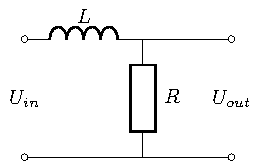
\includegraphics[width=0.5\linewidth]{chem_m/task13a}
	\caption{ФНЧ}
	\label{fig:13a}
\end{figure}

\begin{figure}[h]
	\centering
	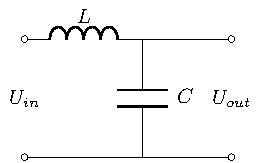
\includegraphics[width=0.5\linewidth]{chem_m/task13b}
	\caption{ФНЧ}
	\label{fig:13b}
\end{figure}

\begin{figure}[h]
	\centering
	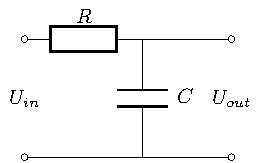
\includegraphics[width=0.5\linewidth]{chem_m/task13c}
	\caption{ФНЧ}
	\label{fig:13c}
\end{figure}


\subsection{Нарисовать и объяснить график $|Z_{BX}|$ последовательного и параллельного колебательных
контуров}

\subsection{Условие безыскажённой передачи сигналов через электрическую цепь}

\subsection{Основные свойства нелинейных цепей}

\subsection{АЧХ и ФЧХ апериодического усилителя}

\subsection{Положительная и отрицательная обратная связь}

\subsection{Критерий Найквиста устойчивости цепи с обратной связью}

\subsection{Рисуем схемы}

\subsection{Динамическая нагрузочная характеристика апериодического усилителя}

\subsection{Правила идеального операционного усилителя}

\subsection{Рисуем схемы}

\subsection{Линейные искажения в резонансном усилителе}

\subsection{Мягкий и жесткий режим возбуждения. Средняя крутизна}

\subsection{Частотные искажения при амплитудном детектировании}
\newpage
\subsection{Спектр на выходе амплитудного детектора}

\subsection{Нарисовать и объяснить график коэффициента передачи преобразователя частоты}

\subsection{Комбинационные частоты приёма}
\end{document}